\documentclass[../BTOF_summary.tex]{subfiles}
 
\begin{document}

\section{Performance Validation}

\subsection{How to Determine the Module Time Resolution}

When considering the time resolution it is important to be aware of which resolution exactly it is you are thinking about.
When determining the time resolution from the time difference variation of the \sipms\ on the two sides of the scintillator it has to be converted to the expected event time resolution.

The measured time difference resolution ($\sigma$) depends on the individual resolutions of the left ($\sigma_L$) and right ($\sigma_R$) \sipm\ arrays. This relation can be easily derived from Equation~\eqref{eq:t_diff} via the propagation of uncertainty.
\begin{align}
	t_{\textit{\tiny diff}} &= t_L - t_R \label{eq:t_diff} \\
	\sigma_{\textit{\tiny diff}} &= \sqrt{ \left( \frac{\partial t_{\textit{\tiny diff}}}{\partial t_L} \; \sigma_L \right)^2 + \left( \frac{\partial t_{\textit{\tiny diff}}}{\partial t_R} \; \sigma_R \right)^2} \nonumber \\
	&= \sqrt{\sigma_L^2 + \sigma_R^2} \label{eq:Delta_t_diff}
\end{align}
Since the \sipms\ used in the left and right array are identical we can assume that the time resolution of the left and right \sipm\ array are the same ($\sigma_L = \sigma_R = \sigma_{L/R}$). This allows us to simplify Equation~\eqref{eq:Delta_t_diff} to
\begin{align*}
	\sigma_{\textit{\tiny diff}} &= \sqrt{2} \; \sigma_{L/R}
\end{align*}
and transform it into
\begin{equation}
	\sigma_{L/R} = \frac{1}{\sqrt{2}} \; \sigma_{\textit{\tiny diff}} \: . \label{eq:Dt_LR}
\end{equation}

%
In order to determine the timing resolution of the detector system, the way it is supposed to function in the experiment, we now however need to understand how the timing of an event in the module is determined. This is done by averaging the left and right \sipm\ signals of the module to receive a single event time ($t_E$).
\begin{equation*}
t_{E} = \frac{1}{2} \left( t_{L} + t_{R} \right)
\end{equation*} 
%
The time resolution of this setup can then be calculated as the propagation of uncertainty from the individual resolutions of the two \sipm\ arrays.
%
\begin{align}
	\sigma_{E} &= \sqrt{ \left( \frac{\partial t_{E}}{\partial t_{L}} \; \sigma_{L} \right)^2 + \left( \frac{\partial t_{E}}{\partial  t_{R}} \; \sigma_{R} \right)^2 } \nonumber \\
	 &= \sqrt{ \left( \frac{1}{2} \; \sigma_L \right)^2 + \left( \frac{1}{2} \; \sigma_R \right) ^2 } \label{eq:Dt_module_long}
\end{align}
%
Again assuming that the resolutions of the two sides are identical Equation~\eqref{eq:Dt_module_long} can be simplified to 
%
\begin{align}
	\sigma_{E} &=  \frac{1}{\sqrt{2}} \; \sigma_{L/R} \, . \label{eq:Dt_module}
\end{align}
If we now substitute $\sigma_{L/R}$ in Equation~\eqref{eq:Dt_module} with the expression in Equation~\eqref{eq:Dt_LR} we receive the statement
\begin{align}
%	\Delta t_{E} &=  \frac{1}{\sqrt{2}} \frac{1}{\sqrt{2}} \Delta t_{\textit{\tiny diff}} \nonumber \\
	\sigma_{E} &= \frac{1}{2} \; \sigma_{\textit{\tiny diff}} \, . \label{eq:time_resolution_Erlangen}
\end{align}

This means that by halving the resolution of the time difference between the left and right side of the scintillator we receive the event time resolution we can expect from the module under normal operation.

\subsection{Time Resolution Surface Scans}
The following scans were performed at the University of Erlangen in collaboration with the group of A. Lehmann.
A more detailed discussion of these measurements can be found in the dissertation of Sebastian Zimmermann\footnote{\url{https://panda.gsi.de/publication/th-phd-2021-001}}.

To ensure a performance as homogeneous as possible over the entire scintillator surface the time resolution was measured at multiple points along the scintillator surface.
This particular test was performed to evaluate the ideal scintillator thickness which, as shown in \fig~\ref{fig:Tchickness_timeRes}, which was determined to be \SI{5}{mm}.

The measurements were performed using a \sr\ source and a small trigger scintillator on a motorized arm, reading out the \sipm\ arrays on the two short sides of the scintillator, to determine the time resolution of the detector module across the entire scintillator surface.
The relevant measurement for a \SI{5}{mm} thick scintillator is shown in \fig~\ref{fig:Time_res_scan_erlangen}.

\begin{figure}[htbp]
    \centering
    \includegraphics*[width=.9\textwidth]{fig/TimeResolution_5mm.pdf}
    \caption{Time resolution surface scan of a \SI{5}{mm} thick scintillator tile.}
    \label{fig:Time_res_scan_erlangen}
\end{figure}

Compiling all measurements into one histogram produces the plot shown in \fig~\ref{fig:timeRes_scan_fit}.
This gives us, when fitted with a Gaussian, the overall average time resolution of \SI{51.1}{ps}, which is well within the design goal of \SI{100}{ps}.

\begin{figure}[htbp]
    \centering
    \includegraphics*[width=.7\textwidth]{fig/run52_widthfit.pdf}
    \caption{Histogram of the time resolution over the entire surface, fit with a gaussian distribution.}
    \label{fig:timeRes_scan_fit}
\end{figure}

\subsubsection*{Voltage Dependence}

The measurements were performed using \hamamatsu\ \texttt{S13360-3050PE} \sipms .
As such they require an operational bias voltage of around \SI{60}{V} or \SI{240}{V} for four \sipms\ in series.
The exact operational voltage optimal for timing measurements needs to be determined based on the \sipms\ used.
To find this voltage the time resolution was measured at different operational bias voltages.
This measurement series is shown in \fig~\ref{fig:BiasScan} and illustrates that close to the optimal voltage a total bias voltage difference of \SI{10}{V} produces an estimated time resolution difference of \SI{1}{ps}.
This shows that not hitting the optimal bias voltage still produces very good detector performance.

\begin{figure}[htbp]
    \centering 
    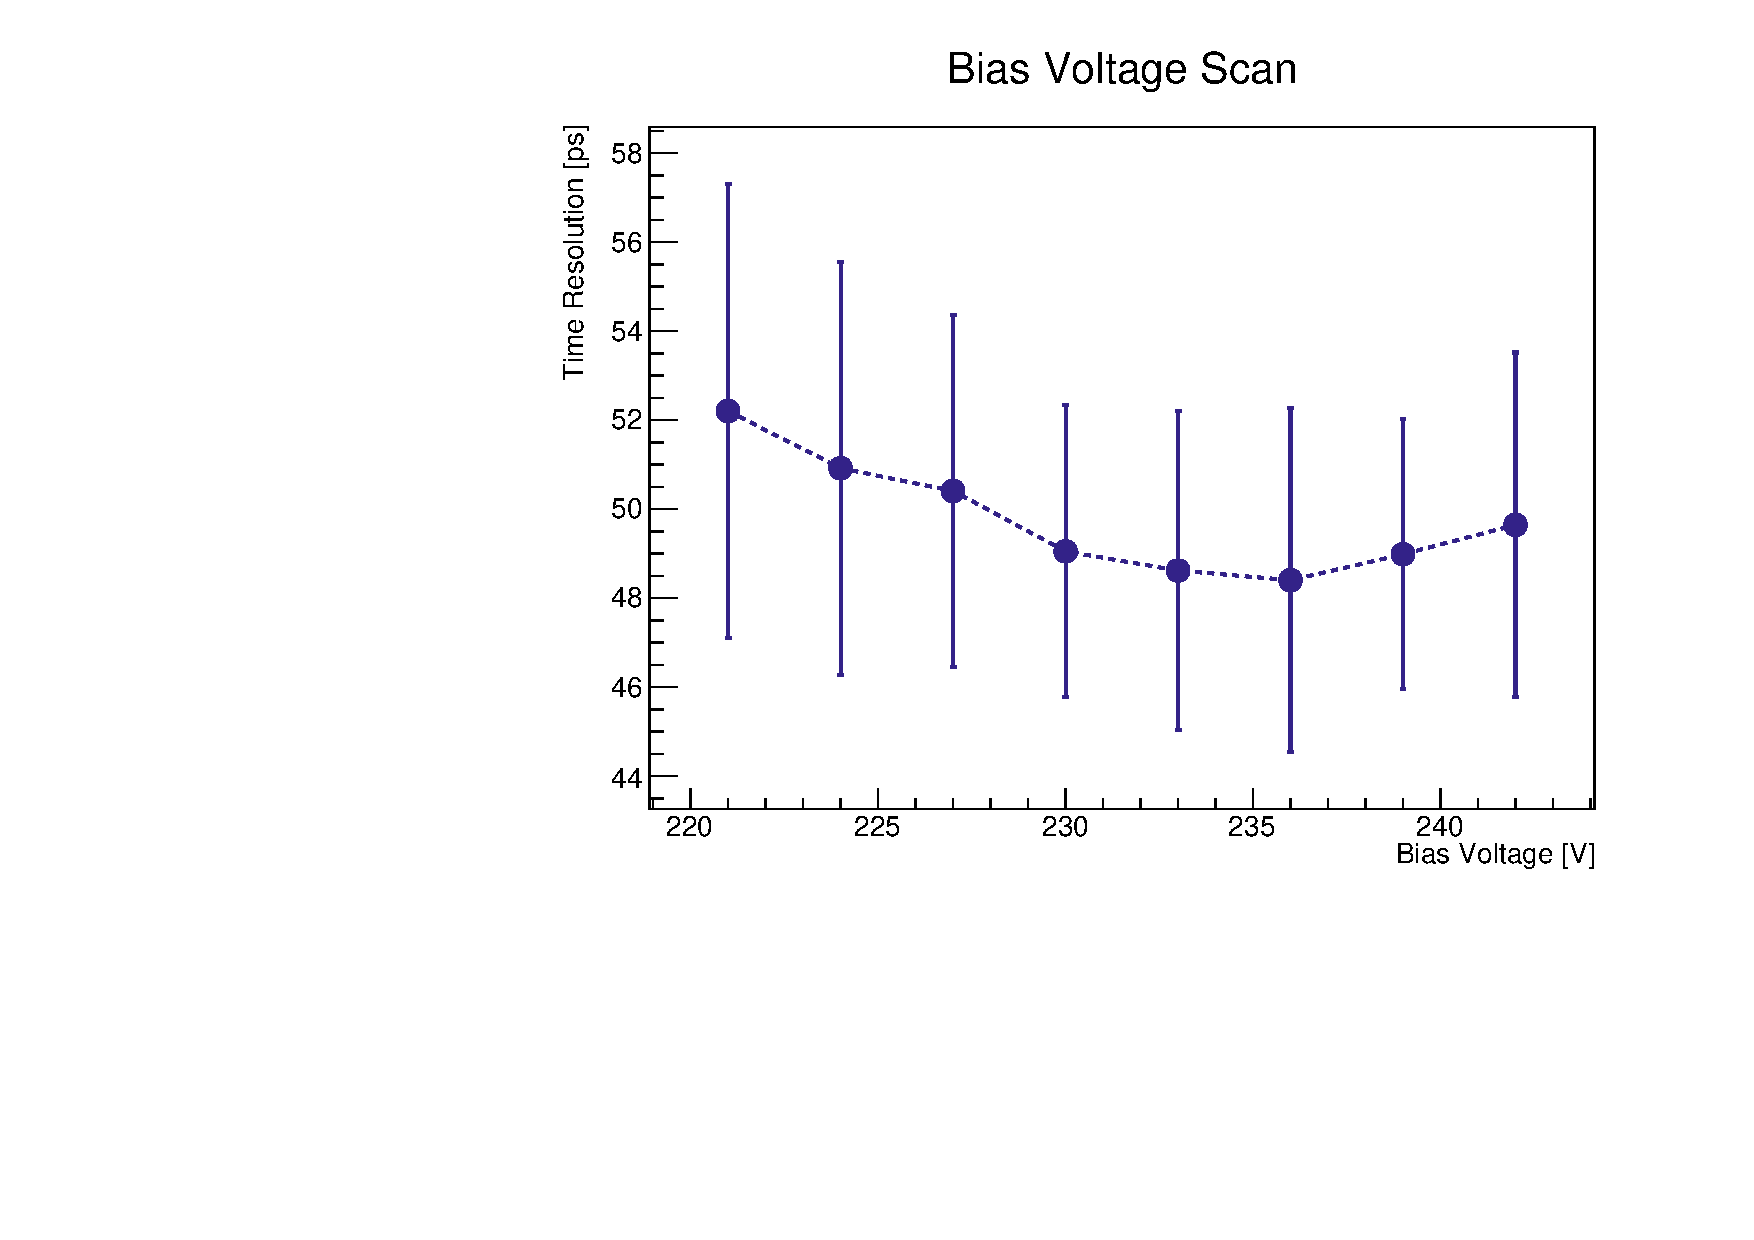
\includegraphics[width=.8\textwidth]{fig/BiasScan.pdf}
    \caption{Bias voltage scan for the serial connection of four \sipms\ in order to determine the optimal operational voltage for time resolution measurements. The time resolution of three points along the scintillator was averaged and the sample standard deviation plotted as the error bars.}
    \label{fig:BiasScan}
\end{figure}

\subsubsection*{Photon Count}

The average photon count along the boards is very homogeneous along the scintillators.
However as expected more photons are detected for events closer to the readout.
The measurements showed that on average one can expect around 100 photons per side per event.

\subsubsection*{Position Resolution}

The position resolution was determined by measuring the timing difference between signals from each side of the scintillator.
Taking the signal timing information of the time resolution scan and simply creating a two dimensional plot of the signal time difference over the entire surface provides a way to gauge the time difference distribution.
The time difference along the short axis, in parallel to the \sipm\ arrays, is almost constant.
Here no information can be extracted.
Taking the time difference along the long axis however reveals an almost linear relation between the signal time difference and the position.
\fig shows a projection of the time difference along the short axis to receive the mean time difference for every position along the long axis.
A linear fit of this distribution reveals a signal speed of \SI{0.12}{mm/ps}.
Combined with the time resolution this produces a position resolution of \SI{12.8}{mm}.

\begin{figure}[htbp]
    \centering
    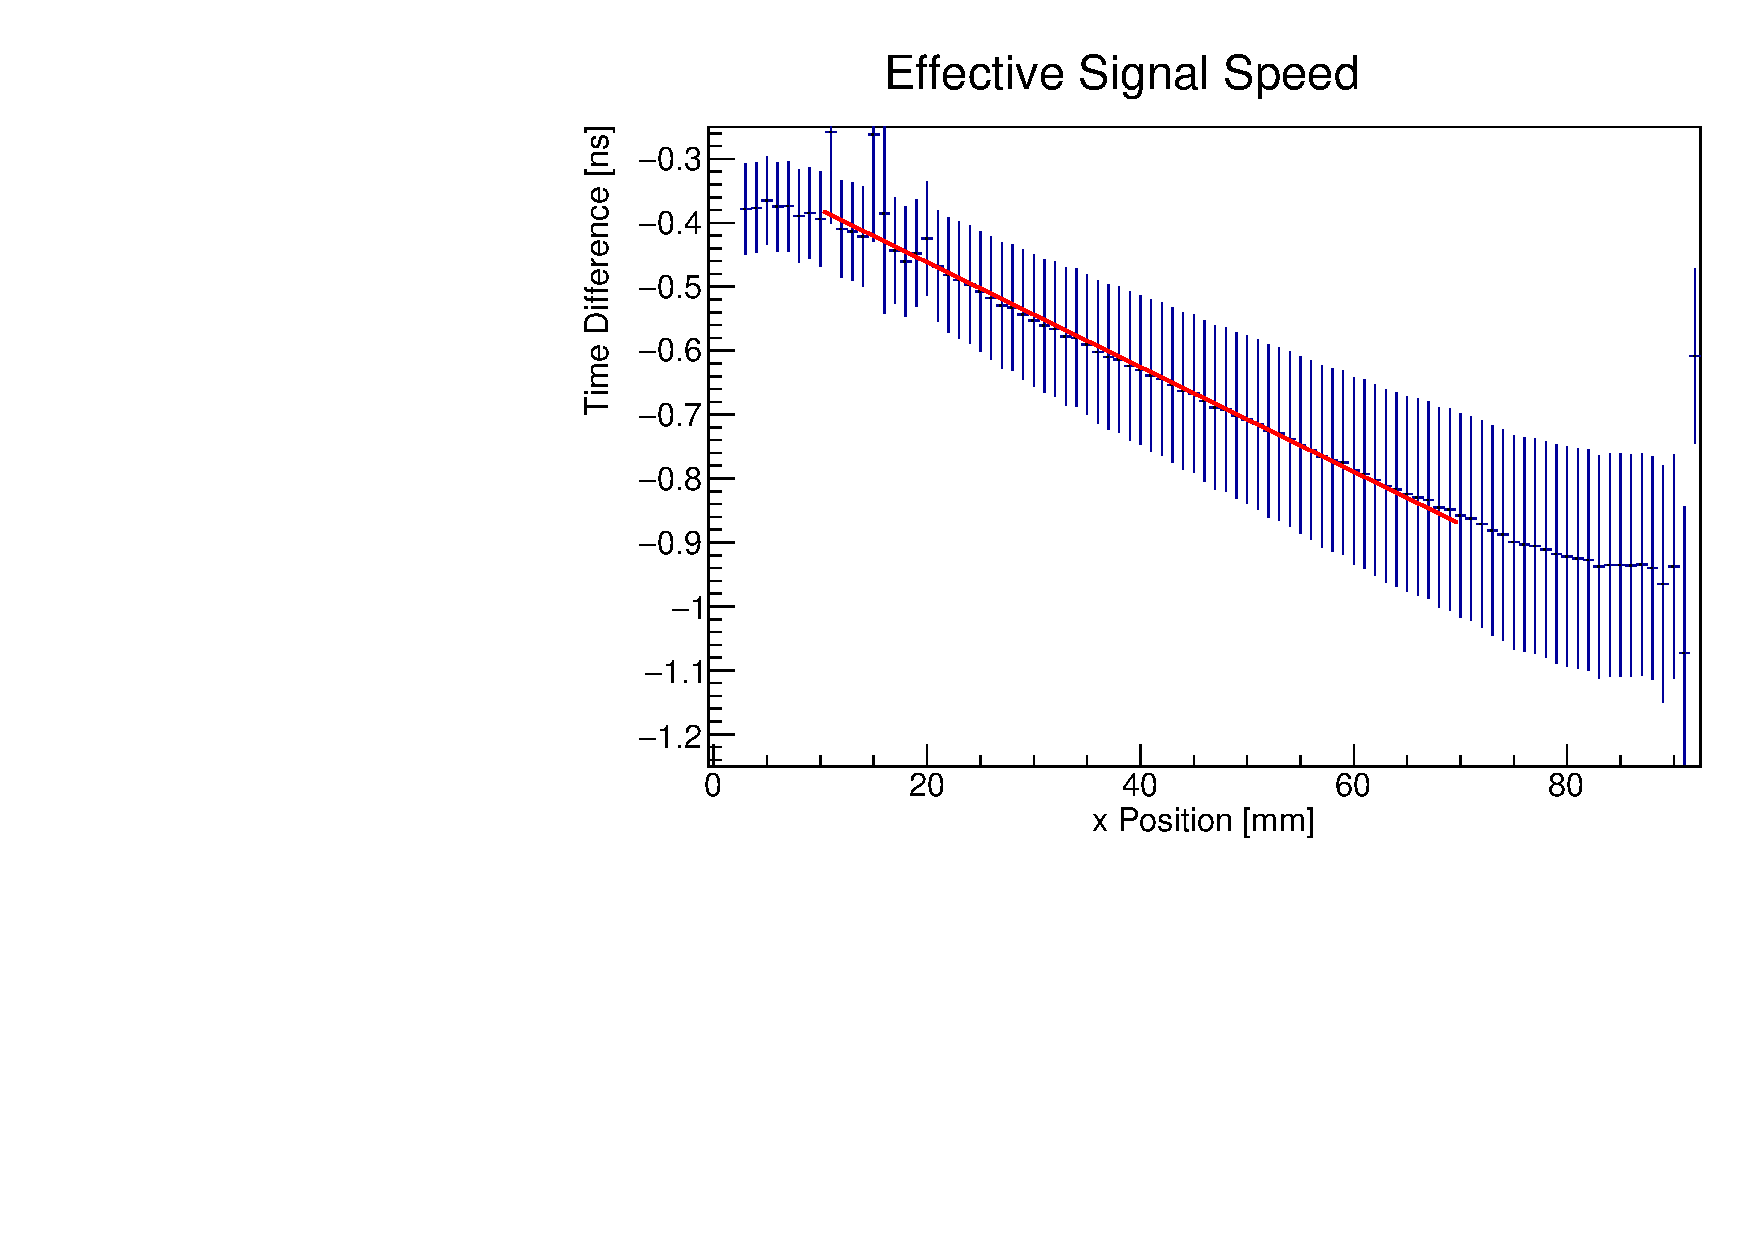
\includegraphics[width=.7\textwidth]{fig/run51_EffectiveSpeed.pdf}
    \caption{The mean time difference depending on the event position along the x axis.}
    \label{fig:positionRes}
\end{figure}

\subsection{CERN Beam tests}
\label{sec:CernBeamTest}

At beam tests in CERN's T9 hall the performance of the \btof\ modules was tested along side the DIRC systems.
Main goal was to establish the detector performance under circumstances closer to the conditions found in \panda\ as well as  studying the influence of adding two additional \sipms\ to the readout array.
Three modules, each with \sipms\ from different manufacturers were tested.
\btof\ module 1 was equipped with \sipms\ by \hamamatsu~(\texttt{S13360-3050PE}).
\btof\ module 2 was equipped with \sipms\ by \ketek~(\texttt{PM3350}).
And \btof\ module 3 was equipped with \sipms\ by \advansid~(\texttt{ASD-NUV3S-P}).

For irradiation a mixed positive beam of mainly protons, kaons and pions was used.
Two ToF stations using \btof\ modules about \SI{30}{m} apart were setup in front of and behind the main detector systems of the DIRC groups.
Due to the large spatial separation of the stations it is possible to resolve two distinct time of flight distributions.
One for the protons and one for kaons and pions presenting the possibility to determine the time resolution for the different particles separately.

To extract the time resolution the distributions were fitted with gaussian distributions.
This does not model the distribution perfectly as it ignores momentum loss effects due to particle interactions in matter.
These interactions produce a Landau distribution as another convolution term of the time of flight spectrum.
It was attempted to incorporate this distortion by fitting the distribution with a Landau-Gauss convolution by using CERN ROOTs languas.C macro.
This however did not yield stable results in the limited time available so further investigations were aborted.
It should be possible to make this work and receive more precise results by tweaking the code.

Since the measured and fitted distributions are convolutions of the time resolution of the individual module resolutions, the single module time resolution has to be extracted.
To do this an overdetermined system of linear equations is created from all time resolution measurements.
Since it is overdetermined it can not be solved analytically but is fitted.
This produces the following result listed in Tables~\ref{tab:Proton_singeTR} and~\ref{tab:Pion_singeTR}.
The results are split into different tables for pions and protons since the particles are affected differently by the matter on its trajectory.

\begin{table}[!htbp]
\caption[Proton peak results of the single detector time resolution fit, listed for all measured beam momenta \emph{p}.]{Proton peak results of the single detector time resolution fit, listed for all measured beam momenta \emph{p}. The statistical fitting errors are omitted since they are all below \SI{0.1}{ps}.}
\label{tab:Proton_singeTR}
\centering
\begin{tabular}{llllll}
\toprule 
p [\si{GeV/c}] & \btof\ 1 [\si{ps}] & \btof\ 2 [\si{ps}] & \btof\ 3 [\si{ps}] & MCP 1 [\si{ps}] & Beam [\si{ps}] \\ 
\midrule
%10  & 64.79 & 78.30 & 51.65 & 98.80 & 111.32 \\
%8 GeV 6 SiPM & 76.11 & 61.48 & 63.68 & 83.21 & 100.79 \\
8  & 77.83 & 59.47 & 72.66 & 84.26 & 103.88 \\
7  & 77.07 & 55.86 & 75.26 & 81.98 & 111.22 \\
%6 GeV 6 SiPM & 76.50 & 63.27 & 62.84 & 82.55 & 114.77 \\
6  & 76.85 & 55.24 & 76.70 & 85.22 & 119.48 \\
5  & 75.56 & 71.37 & 61.12 & 80.24 & 124.98 \\
4  & 69.72 & 62.26 & 71.00 & 84.77 & 156.27 \\
%4 GeV 4 SiPM & 70.71 & 77.75 & 61.59 & 82.04 & 154.65 \\
%4 GeV 6 SiPM & 68.06 & 66.69 & 64.52 & 86.66 & 153.81 \\
3  & 65.66 & 65.77 & 66.53 & 88.90 & 225.98 \\
\midrule
\textbf{Mean} & 73.8 $\pm$ 5.2 & 61.7 $\pm$ 7.5 & 70.5 $\pm$ 6.8 & 84.2 $\pm$ 4.5 & --------- \\
\bottomrule
\end{tabular} 
\end{table}

\begin{table}[!htbp]
\caption[Pion peak results of the single detector time resolution fit, listed for all measured beam momenta \emph{p}.]{Pion peak results of the single detector time resolution fit, listed for all measured beam momenta \emph{p}. The statistical fitting errors are omitted since they are all below \SI{0.1}{ps}.}
\label{tab:Pion_singeTR}
\centering
\begin{tabular}{llllll}
\toprule 
p [\si{GeV/c}] & \btof\ 1 [\si{ps}] & \btof\ 2 [\si{ps}] & \btof\ 3 [\si{ps}] & MCP 1 [\si{ps}] & Beam [\si{ps}] \\ 
\midrule
%10  & 74.65 & 43.91 & 82.89 & 91.58 & 107.86 \\
%8 GeV 6 SiPM & 78.32 & 53.00 & 70.89 & 81.13 & 94.76 \\
8  & 78.84 & 53.66 & 77.05 & 83.32 & 97.26 \\
7  & 79.82 & 52.99 & 77.31 & 79.30 & 102.57 \\
%6 GeV 6 SiPM & 81.18 & 57.24 & 68.37 & 77.96 & 100.97 \\
6  & 81.91 & 51.96 & 78.96 & 80.37 & 105.09 \\
5  & 81.91 & 63.82 & 68.97 & 73.75 & 98.20 \\
4  & 79.16 & 55.56 & 76.35 & 76.03 & 102.37 \\
%4 GeV 4 SiPM & 80.48 & 68.80 & 71.44 & 72.49 & 102.41 \\
%4 GeV 6 SiPM & 78.79 & 60.01 & 70.78 & 77.04 & 97.43 \\
3  & 78.90 & 56.71 & 74.41 & 77.38 & 114.40 \\
\midrule
\textbf{Mean} & 80.1 $\pm$ 1.5 & 55.8 $\pm$ 4.3 & 75.5 $\pm$ 3.5 & 78.4 $\pm$ 3.4 & --------- \\

\bottomrule
\end{tabular} 
\end{table}

The time resolution however was expected to be independent of particle type, and a close to constant value was expected for all detector modules since they are all equipped with functionally the same hardware only using different \sipm\ models by different manufacturers.
The data shows different absolute results for protons and pions with a similar trend between the measurements.
These results suggest that the \btof\ module 2 performs the best, followed by \btof\ module 3 and then module 1.
However large correlations between the modules especially the ones situated in a single station distort the results.
Nonetheless the measurements showed that the detector performs well below the design goal of \SI{100}{ps} even under less controlled circumstances.

\subsubsection*{Truncation of Scintillator}
    
As mentioned previously the scintillator shape was slightly altered compared to the design in the TDR in order to fit small pillars in between the scintillator tiles.
These pillars serve as mounting points for the split \railboard\ and offer guidance to the scintillator tiles holding them in place without applying any pressure.

The performance impact of this change was studied using a pulsed laser on a mechanized arm, comparing time resolution measurements of cut and uncut scintillator tiles.
For this a partial scan of two scintillator tiles was performed measuring the time resolution of one half on the scintillator.
As shown in \fig~\ref{fig:Surface_Scan_cutUncut} no time resolution worsening can be seen when removing scintillator material from the corners.
In the contrary the measurements show a time resolution improvement for the scintillator with the cut corners.
This however is most likely due to systematic errors of the measurements and not a general performance improvement due to the new geometry since the improvement is constant across the surface.

\begin{figure}[htpb]
	\centering
	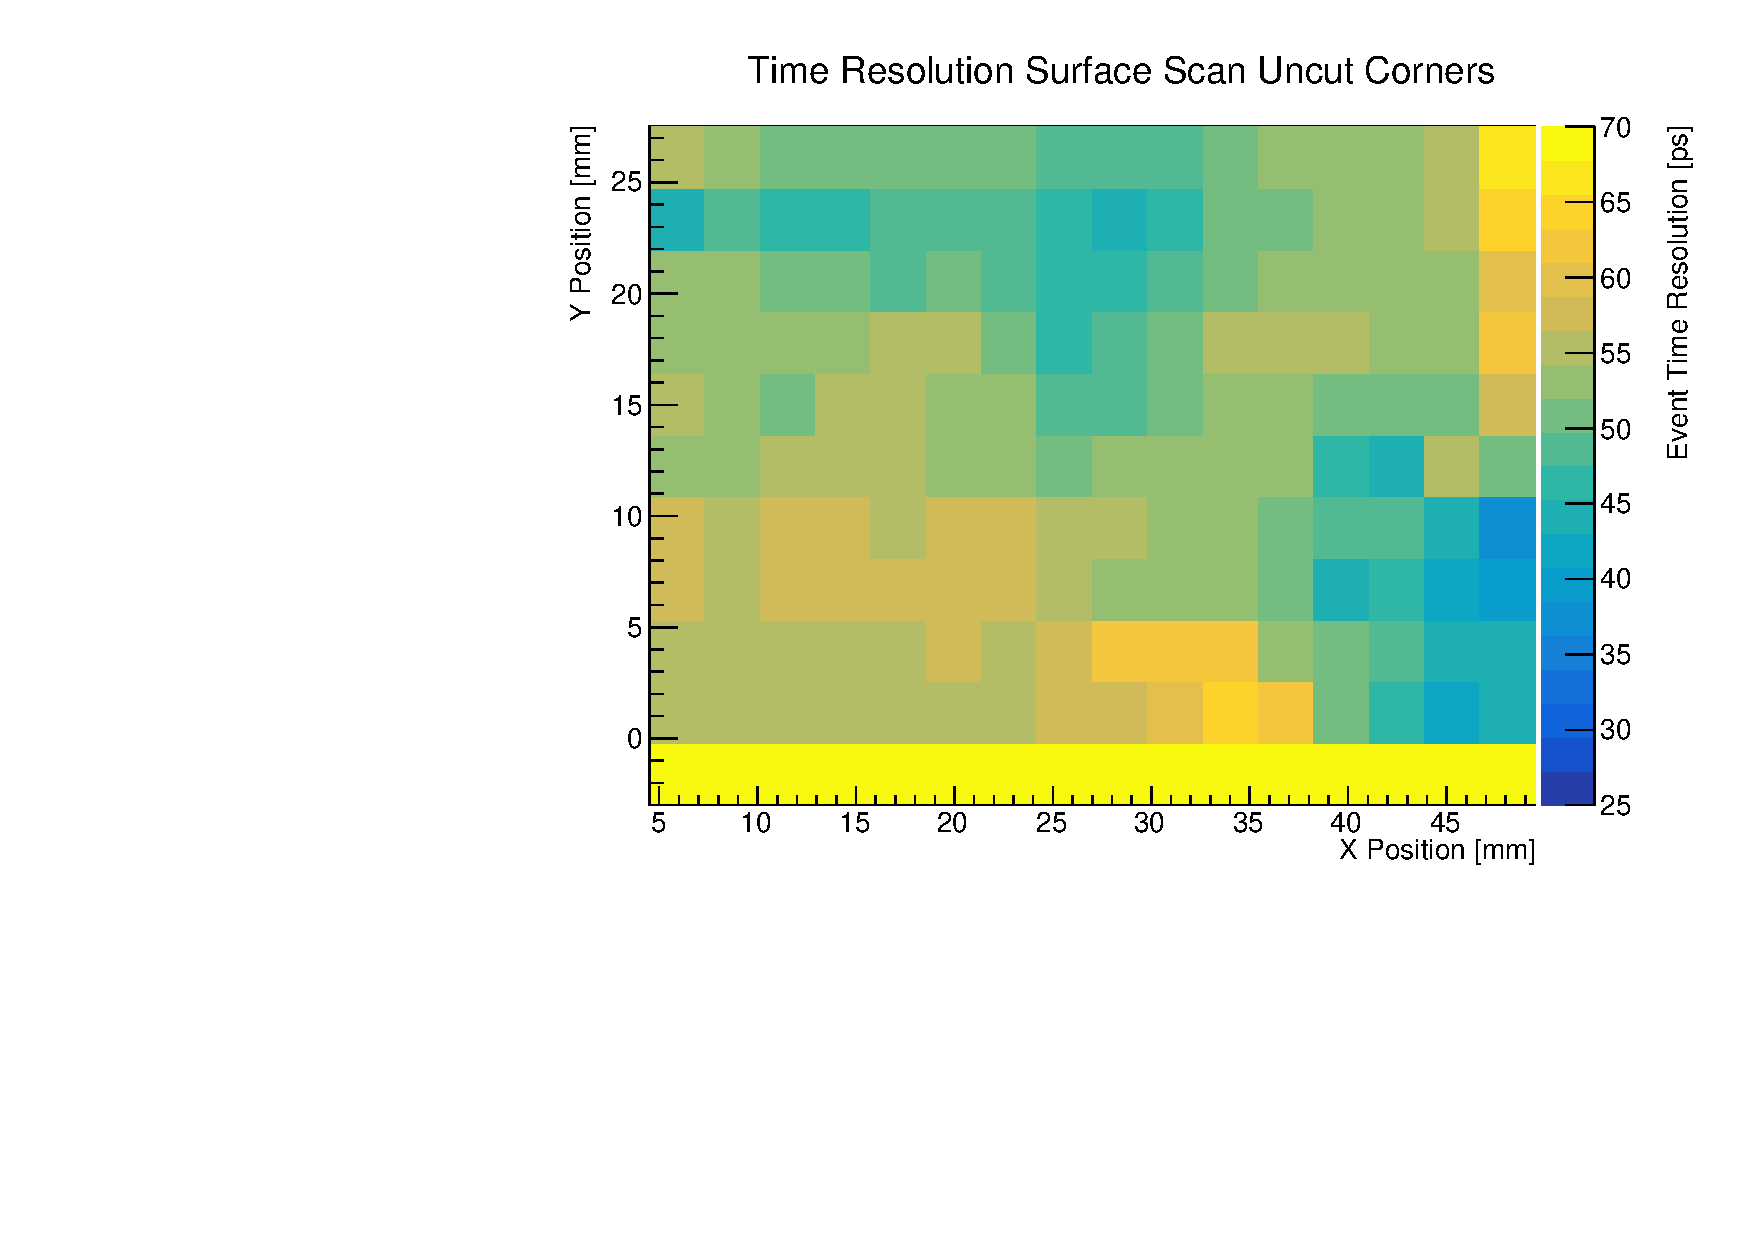
\includegraphics[width=.49\textwidth]{fig/Time_Resolution_Surface_Scan_Uncut_Corners.pdf}
	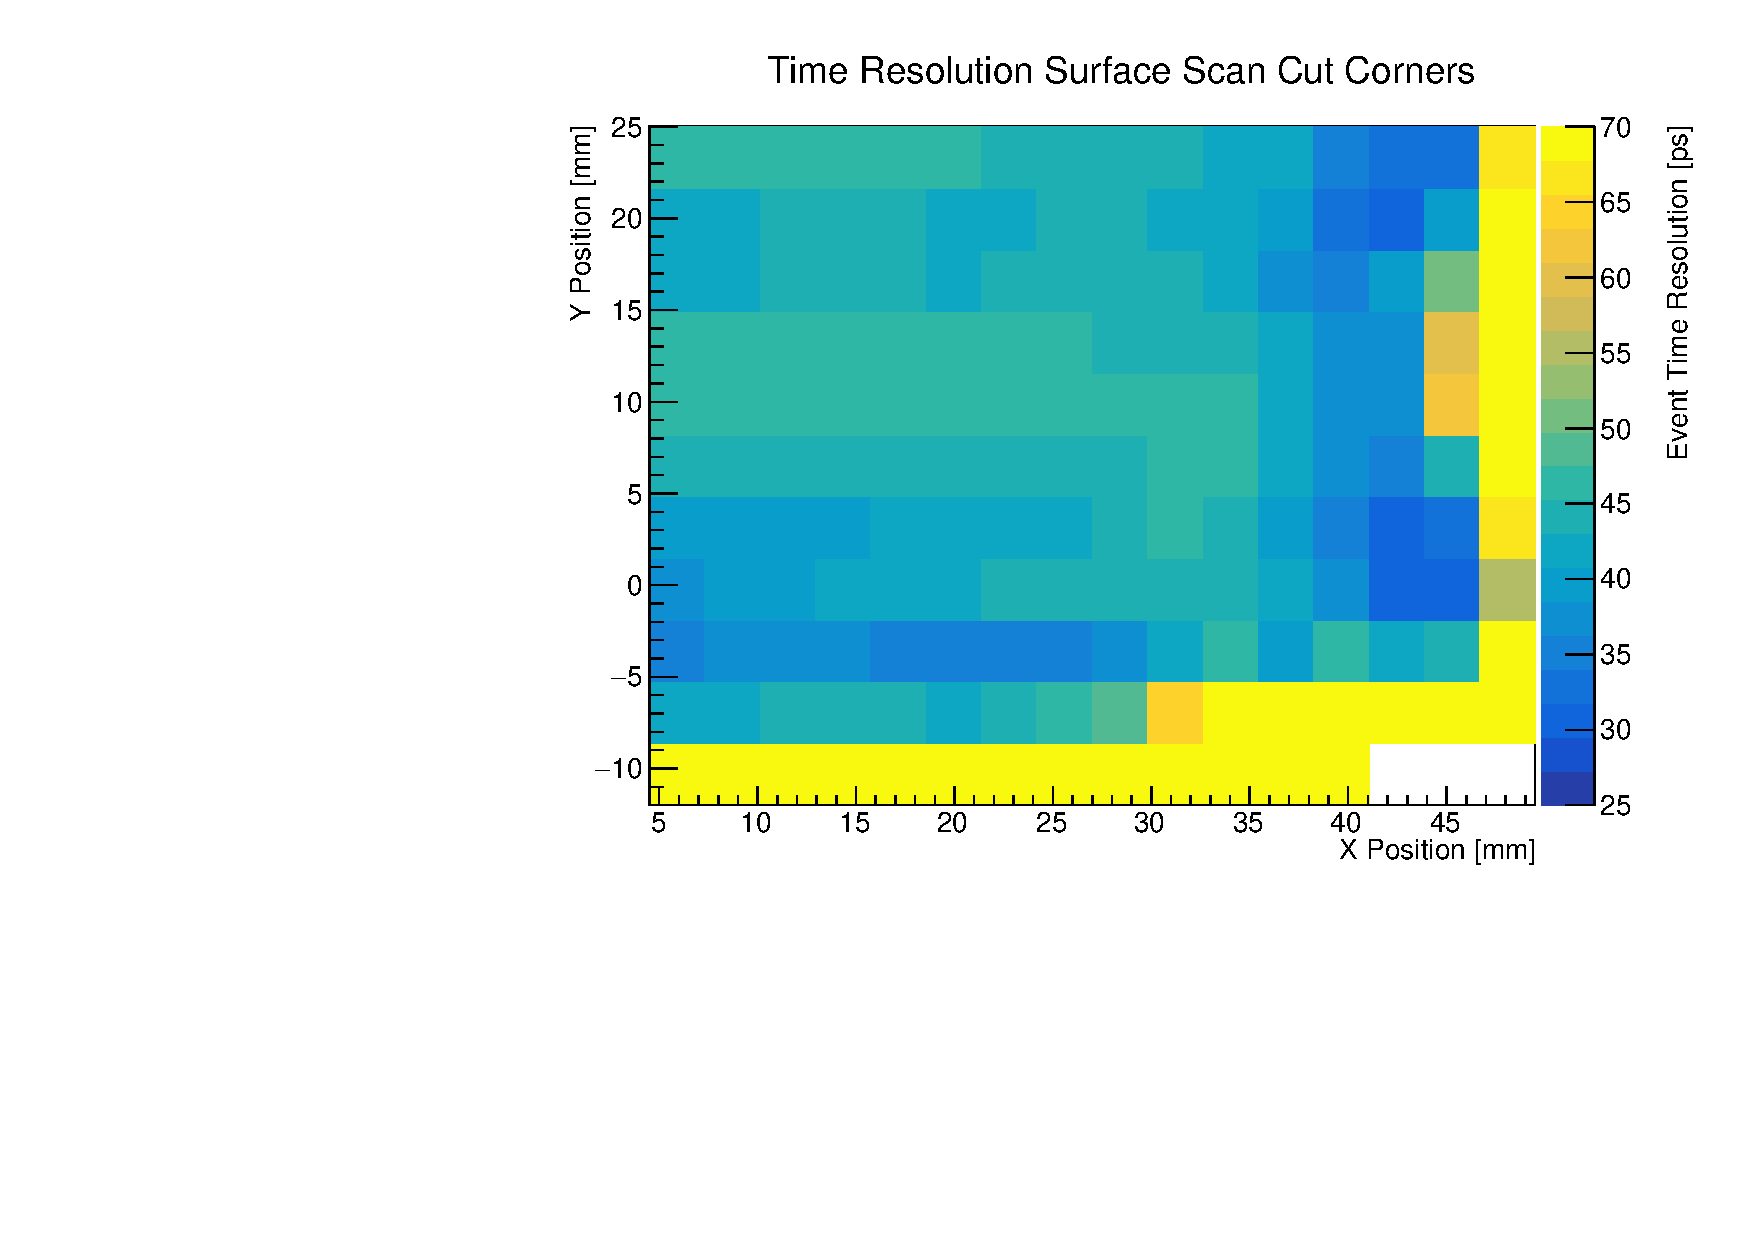
\includegraphics[width=.49\textwidth]{fig/Time_Resolution_Surface_Scan_Cut_Corners.pdf}
	\caption{Comparison of the partial time resolution surface scan achieved with a scintillator tile of old dimensions (left) and new dimensions with a cut corner (right). In each instance half the tile was scanned with the edge at around x=\SI{50}{mm}.}
	\label{fig:Surface_Scan_cutUncut}
\end{figure}


\end{document}